%!TEX root = main.tex
\section{Dataset}
På de følgende sider vil vi gennnemgå vores dataset. Vi vil vise de basale statistikker over dataet for hver af de perioder vi har arbejdet med og gennemgå afvigelser. Vi vil også gennemgå hvordan vi forholder os til disse afvigelser og hvordan vi lavede datacleaning. \\
Til sidst vil vi runde afsnittet af med en del-konlusion. 

Vores data stammer fra Sony's Lifelog\cite{sonyLifeLog} som, navnet antyder, er en mobil Lifelog app som logger ens aktiviteter i løbet af dagen. Heri logger den bla. aktivitet i apps og geolokation. Vores dataset stammer fra denne app, indsamlet fra Sony medarbejdere og, som det fremkommer senere, henover forskellige perioder i 2015. % over 3 måneder\footnote{September 2015 - November 2015} fordelt på 80 lande. 

Vi har valgt at dele datasættet op i to dele, for overblikkets skylde: En \textbf{geolokation del} og en \textbf{app og homophily del}.

\subsection{Geolokation del}
Denne del af datasættet beskriver geolokationerne for hvor en bruger har været. Det beskriver præcis hvor, hvornår og hvor længe brugeren har været det pågældende sted. Hver gang brugeren skifter lokation (defineret ud fra latitude og longitude), bliver der logget en lokations opdatering med følgende oplysninger:
\begin{enumerate}
\item \texttt{\textbf{timestamp\_seen}}\\Millisekunder siden brugerens systems epoch, da den pågældende lokations opdatering bliver logget. 
\item \texttt{\textbf{id}}\\Lokations id repræsenteret som en streng. 
\item \texttt{\textbf{useruuid}}\\Brugerens unikke id repræsenteret som en streng
\item \texttt{\textbf{start\_time}}\\Tid for hvornår brugeren går ind i en lokation. Repræsenteret som ISO8601 time stamp med timezone
\item \texttt{\textbf{end\_time}}\\Tid for hvornår brugeren går ud af en lokation. Repræsenteret som ISO8601 time stamp med timezone
\item \texttt{\textbf{name}}\\Navnet på byen hvor brugeren befinder sig, når lokations opdateringen bliver logget
\item \texttt{\textbf{area}}\\Navnet på området hvor brugeren befinder sig, når lokations opdateringen bliver logget. F.eks. Skåne i Sverige
\item \texttt{\textbf{country}}\\Navnet på landet hvor brugeren befinder sig, når lokations opdateringen bliver logget
\item \texttt{\textbf{region}}\\Navnet på regionen hvor brugeren befinder sig, når lokations opdateringen bliver logget. F.eks. EU
\item \texttt{\textbf{latitude}}\\Latitude for lokationen. Latitude har en præcition på ca 15 cifre, hvilket svarer til 0.1 nanometer [KILDE!!!]. Denne præcition er skal man dog ikke tage så højtidligt, da de fleste mobil GPS'er har en fejl margen på maks 30 meter \cite{NAV:8292634}.  
\item \texttt{\textbf{longitude}}\\Longitude for lokationen. Latitude har en præcition på ca 15 cifre, hvilket svarer til 0.1 nanometer. Vedr. præcition, gælder det samme som ved latitude
\item \texttt{\textbf{altitude}}\\Altitude repræsenteret i mm. Dette bliver beregnet af telefonens gyroskop samt GPS
\item \texttt{\textbf{accuracy}}\\Accuracy repræsenteret i mm. Accuracy er hvor nøjagtigt man kan regne med GPS'en er i den pågældene lokations opdatering. Værdien fortæller at brugeren med sikkerhed er i pågældende sted, indenfor denne distance som accuracy er. Jo lavere værdi, jo bedre. Dette styres af telefonens styresystem og GPS
\item \texttt{\textbf{devices}}\\Devices er repræsentet som et array med name, type og id. Type er hvilken type device (f.eks. Phone), name er navnet på det device og id er devices unikke id. 
\end{enumerate}

Nogle af overstående oplysninger er ikke relevante for vores problemstilling. Dette gør vi kan skære disse fra og vi ender dermed at have følgende oplysninger (fra nu af kaldt  attributter) at arbejde med: 

\begin{itemize}
\item \texttt{useruuid}
\item \texttt{start\_time}
\item \texttt{end\_time}
\item \texttt{name}
\item \texttt{area}
\item \texttt{country}
\item \texttt{region}
\item \texttt{latitude}
\item \texttt{longitude}
\item \texttt{altitude}
\item \texttt{accuracy}
\end{itemize}

Disse oplysinger har vi valgt, da de mere eller mindre er vigtige eller interssante i forhold til vores problemstilling. \texttt{useruuid} er vigtig for at kunne skelne brugerene fra hinanden, \texttt{start\_time} og \texttt{end\_time} er vigtige, da de fortæller hvornår/hvor længe brugeren har været i den pågældende lokation. \texttt{country} er til nemt at kunne filtrere brugerene, hvor \texttt{name}, \texttt{area} og \texttt{region}, ikke er særlige vigtige men kunne være interessant at kigge på. \texttt{latitude} og \texttt{longitude} er meget væsentlige, da de fortæller nok det mest vigtigste, nemlig hvilken lokation brugeren befinder sig. \texttt{accuracy} kan fortælle os i for høj grad vi kan bruge den pågældene lokations opdatering, mens \texttt{altitude} kunne være interessant at at kigge på mht. fin-filtrering. 

Vi har kigget på data fra flere perioder. Vi vil nu beskrive hvordan hver periode ser ud mht. distributioner mm. Disse perioder er: 
\begin{itemize}
\item Periode 1: September 2015 - November 2015
\item Periode 2: ??????????
\end{itemize}

\subsubsection{Periode 1}
Denne periode er over 3 måneder: fra september - november 2015. Vi vil gennemgå hvordan datasættet så ud i denne periode. 
Henover denne periode blev der indsamlet 2.665.893 lokations opdateringer fordelt på 1586 brugere

I Table \ref{tab:stat_geo_p1} ses statistic summary af \texttt{accuracy}, \texttt{altitude}, \texttt{name} og \texttt{country}.
Vi kan se i tabellen at der er nogle ugyldige værdier både accuracy og altitude. De ugyldige værdier viser sig i form af negative værdier. Ud af de mange lokations opdaterings er der kun 20 hvor accuracy er negativ hvilket svarer til knapt en 1000 del procent. Altitude har også nogle negative værdier. Her er negative værdier sådan set ikke ugyldige, men dog sjældne og unormale. Hvis vi kigger på antal lokations opdaterings der har en negativ altitude på mindre end -50.000 (-50m), er der 9. Ved mindre end -10.000 (-10m) er der 14.

\begin{table}[H]
        \centering
        \small
        \setlength\tabcolsep{2pt}
        \begin{tabular}{|c|c|c|c|c|}
            \hline
                         & Accuracy           & Altitude    & Name   & Country  \\[-3pt]% compensate for extrarowheight
                         &  (mm)              & (mm)        & (city) &          \\
            \hline
                 Unique  &                    &             & 19.344 & 80        \\
                 entries &                    &             &        &           \\
            \hline
                 Min     &  -2.147.483.500    & -5.086.000  &        &           \\
                         &                    &             &        &           \\
            \hline
                 Max     &  500.000           & 17.211.698  &        &           \\
                         &                    &             &        &           \\
            \hline
                 Mean    & 35.249             & 105.030     &        &           \\
                         &                    &             &        &           \\
            \hline
                 Std.    & 3.672.390          & 403.966     &        &           \\
                 dev.    &                    &             &        &           \\
            \hline
        \end{tabular}
        \caption{Statistic summary of datset in periode 1} %add this between 'caption' and '{...' for new text in listing of tables: [New caption text only for listing of tables]
        \label{tab:stat_geo_p1}
\end{table}



Da vi endnu ikke bruger altitude, vælger vi at se bort fra disse sjældne værdier og beholder de berørte opdateringer. Dog påvirker accuracy latitude og longitude, som er vores vigtigste attribut, så disse fjerner vi. Herudover fjerner vi også de lokations opdateringer hvor accuracy er over 100.000 (100m) pga. vores binning (se mere i section \ref{ssec:binning}, s. \pageref{ssec:binning}), da disse alligevel har en sandsynlighed for at være udenfor vores binning. 
%Dette gjorde vi kom ned på at have 2.274.333 lokations opdateringer i vores datasæt. 

Efter dette, så quantilerne af accuracy ud som man kan se på Tabel \ref{tab:acc_quantiles}. 
 \begin{table}[htbp]
        \centering
        \small
        \setlength\tabcolsep{2pt}
        \begin{tabular}{|c|c|c|}
            \hline
                         & Accuracy      \\[-3pt]
            \hline
                 Minimum &  3,000       \\
            \hline
                 Q1      &  10,000   \\
            \hline
                 Median  &  23,000    \\
            \hline
                 Mean    &  26,894.356    \\
            \hline
                 Q3      &  39,000      \\
            \hline
                 Maximum &  100,000   \\
            \hline
                 IQR     &   29,000     \\
            \hline
                Std. deviation  &  20,290.826   \\
            
        \end{tabular}
        \caption{Quantiles of accuracy after cleaning} %add this between 'caption' and '{...' for new text in listing of tables: [New caption text only for listing of tables]
        \label{tab:acc_quantiles}
\end{table}

Vi kan se på medianen og mean, at de fleste brugere har lav værdi i accuracy - hvilket er godt! Hvis vi antager at det følger en normalfordeling, kan vi ud fra standard deviation udlede, at 95\% af brugerne har en accuracy mellem 6,603.53 og 47,185.182. Dette viser at der er nogle få brugere med meget høje værdier i accuracy, hvor max er 100,000. Medianen og mean svarer til henholdsvis 23m og 26.89m og 95\% standard deviation er på mellem 6.6m og 47.19m hvilken er en fin accuracy. 

Som Tabel \ref{tab:stat_geo_p1} viser, har vi at gøre med 80 unikke lande. Til at starte med lå dette tal på 74. Det viste sig, at der var en masse lokations opdaterings hvor landet ikke var blevet logget. Her var landet blot repræsenteret med en tom streng. Dette var tilfældet i så stor en del af dataet, at landet med en tom streng, var det andet mest representerede land i dataet med lidt over 500.000 lokations opdaterings. 
Dette var et problem som vi løste, ved at udfører omvendt geolokation. For næsten alle de 500.000 lokations opdaterings, var latitude og longitude til stede, så vi kunne ved hjælp af et API\cite{reversegeocode} slå landet op på bagrund af latitude og longitude, og herefter indsætte det i dataet. 
Dette gjorde at vi gik fra over 500,000 lokations opdaterings hvor landet ikke var til stede, til blot 130 lokations opdaterings. I samme omgang gik vi fra 74 lande til 80 (inkl. land med tom streng)

Vi kigger herefter på, hvordan lokations opdateringerne er distribueret over hvert land. På figur \ref{fig:country_dist} kan vi se at landet med en tom streng, røg godt ned på listen, mens Sverige og Japan topper listen. 
% \begin{table}[htbp]
%         \centering
%         \small
%         \setlength\tabcolsep{2pt}
%         \begin{tabular}{|c|c|c|c|c|c|c|c|c|c|c|}
%             \hline
%                          & Latitude/  &   start             & end               & Accuracy           & Altitude    & Name   & Country & Region             & Area          \\[-3pt]% compensate for extrarowheight
%                          & longitude  &  time               & time              &  (mm)              & (mm)        & (city) &         & (Europe, Asia...)  & (Area/state)  \\
%             \hline
%                  Unique  &            &                     &                   &                    &             & 19.344 & 80      &                    &               \\
%                  entries &            &                     &                   &                    &             &        &         &                    &               \\
%             \hline
%                  Min     &            &   2015-08-09        &                   &  -2.147.483.500    & -5.086.000  &        &         &                    &               \\
%                          &            &   22:25:33.766+02   &                   &                    &             &        &         &                    &               \\
%             \hline
%                  Max     &            &                     &   2015-12-01      &  500.000           & 17.211.698  &        &         &                    &               \\
%                          &            &                     &  01:00:22.711+01  &                    &             &        &         &                    &               \\
%             \hline
%                  Mean    &            &                     &                   & 35.249             & 105.030     &        &         &                    &               \\
%                          &            &                     &                   &                    &             &        &         &                    &               \\
%             \hline
%                  Std.    &            &                     &                   & 3.672.390          & 403.966     &        &         &                    &               \\
%                  dev.    &            &                     &                   &                    &             &        &         &                    &               \\
%             \hline
%         \end{tabular}
%         \caption{Overview and statistic summary of geolocation dataset} %add this between 'caption' and '{...' for new text in listing of tables: [New caption text only for listing of tables]
%         \label{tab:stat_geo}
% \end{table}


\begin{figure}[H]
    \centering
    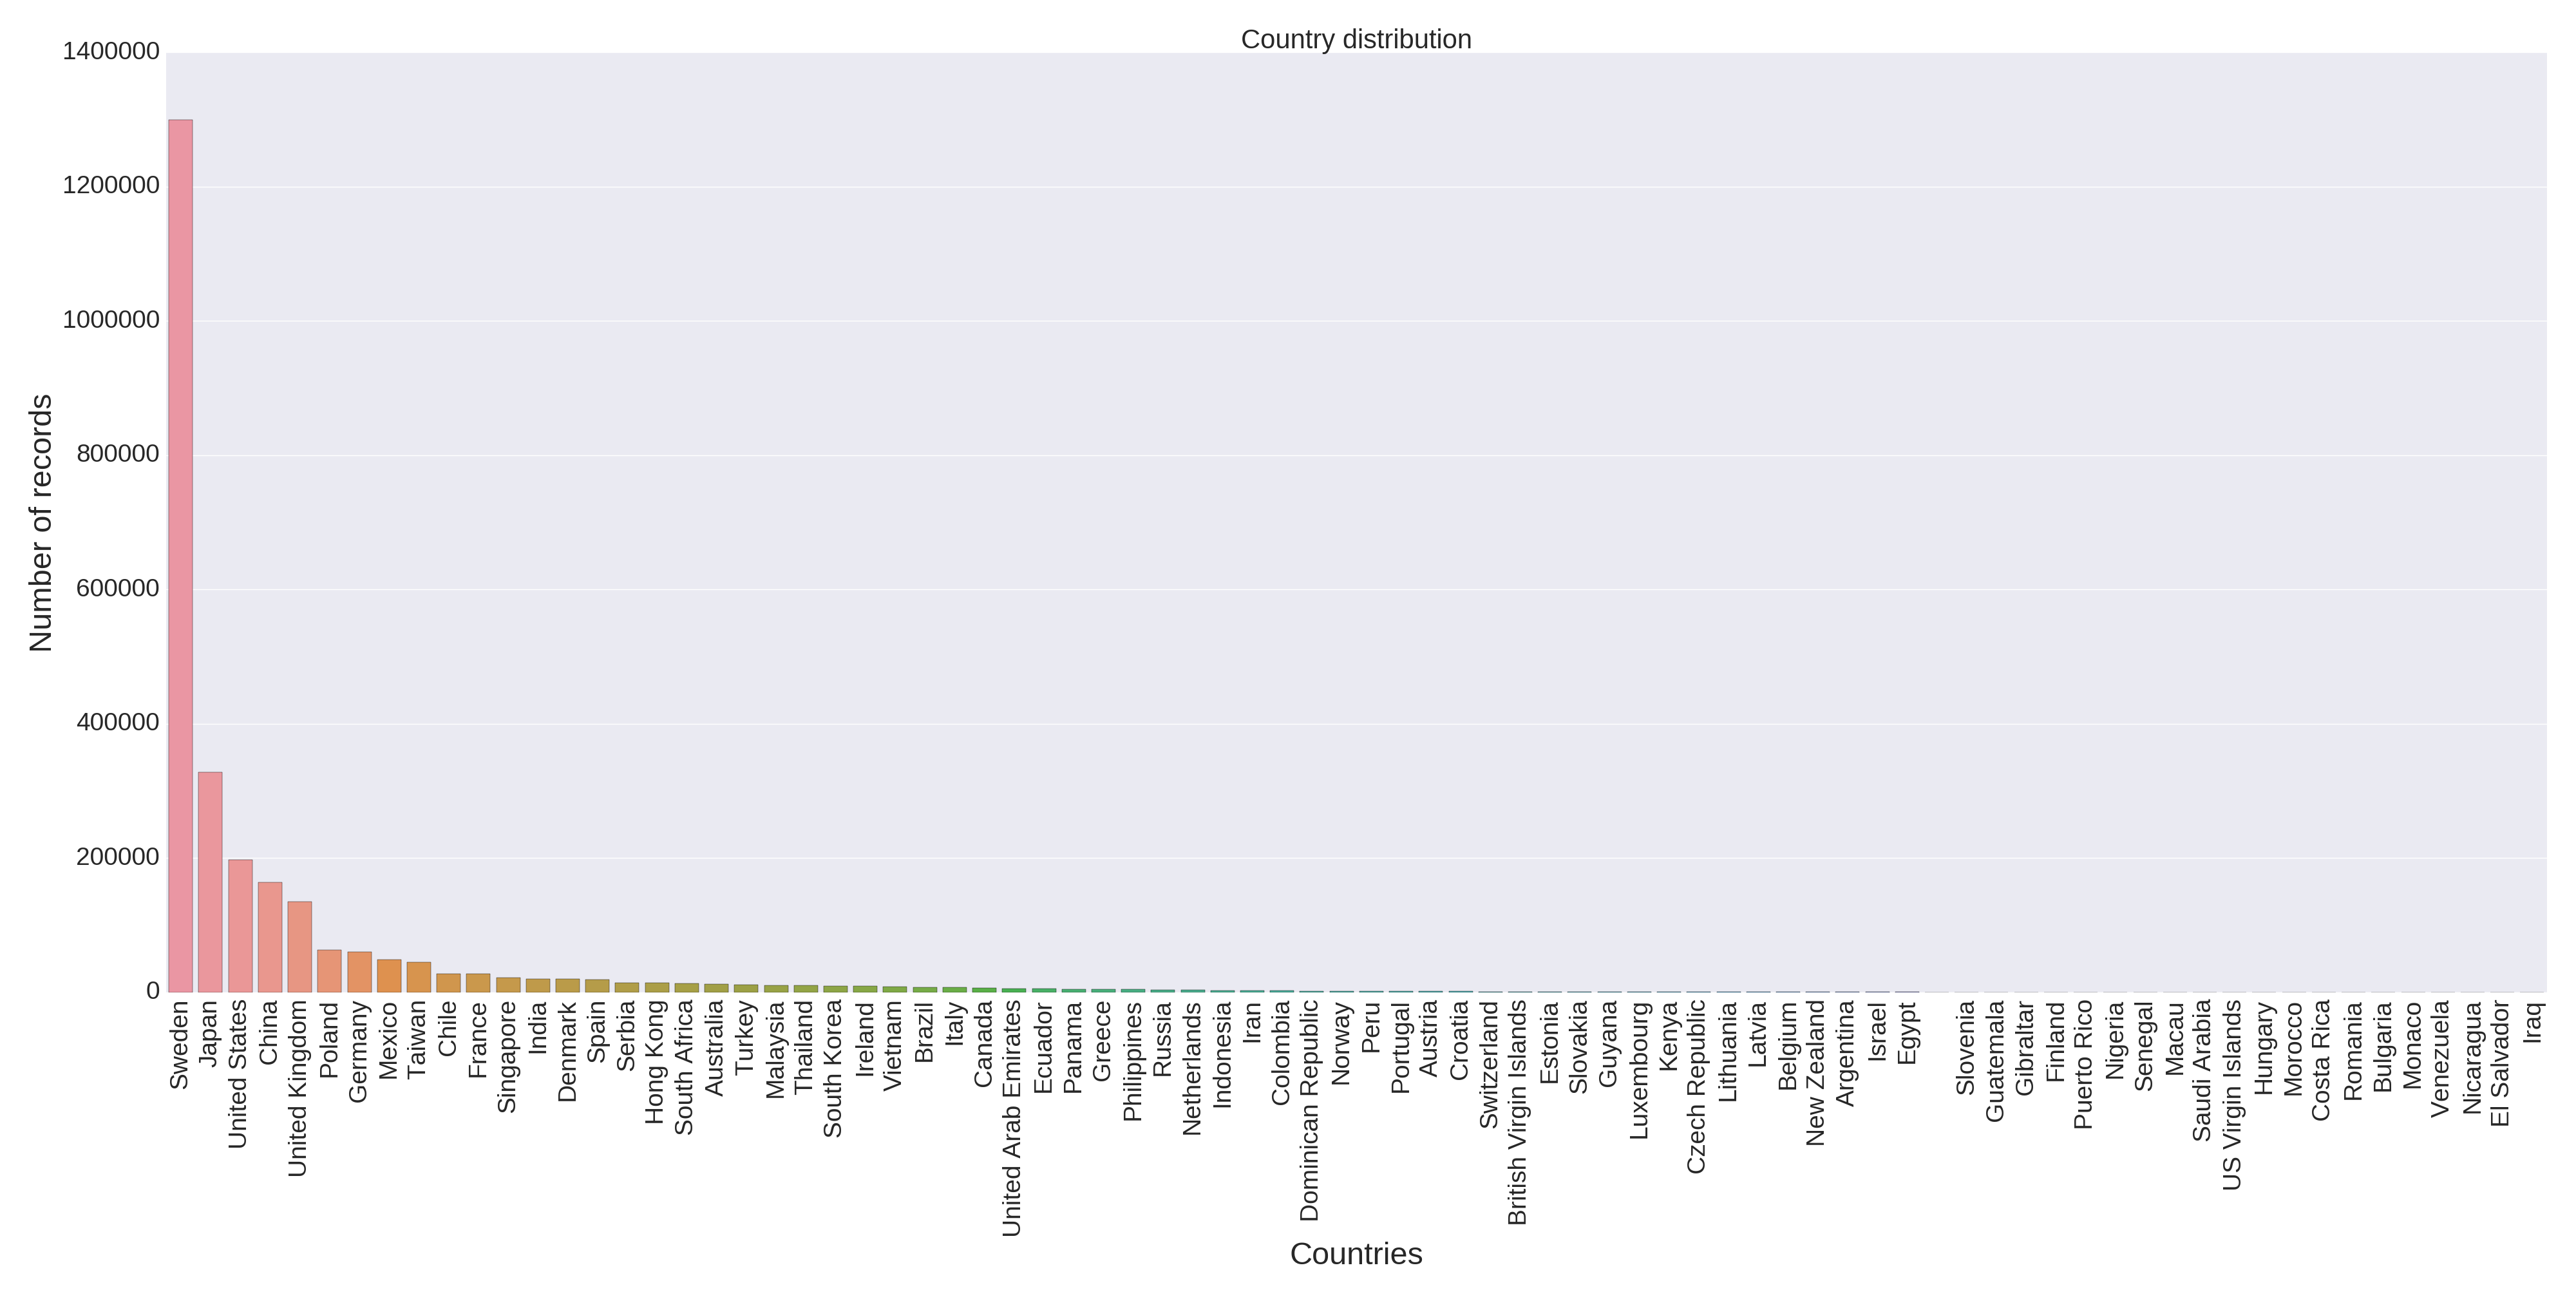
\includegraphics[scale=0.18]{country_distribution}
    \caption{Distribution for number of lokations opdaterings between countries}
    \label{fig:country_dist}
\end{figure}

På baggrund af Figure \ref{fig:country_dist}, har vi valgt at gå videre med endten Sverige eller Japan. Derfor vil vi nu sammeligne data for de to lande. 
På Figure \ref{fig:country_cd} ser vi at der er en stor del af brugerne både i Japan og Sverige, som har meget få lokations opdateringer henover hele perioden. Over en tredje del af brugerne i begge lande, har maximalt 109 og 161 opdateringer over 3 måneder for henholdsvis Japan og Sverige. Da opdateringerne kommer hver gang brugeren skifter lokation, betyder dette at mange af brugerene er meget stillestående eller også har de slukket mobilen. Begge disse scenarier tegner ikke godt for vores mål, da det giver sig selv at der skal være nogle data for at finde co-occurences. 


\begin{figure}[H]
    \centering
    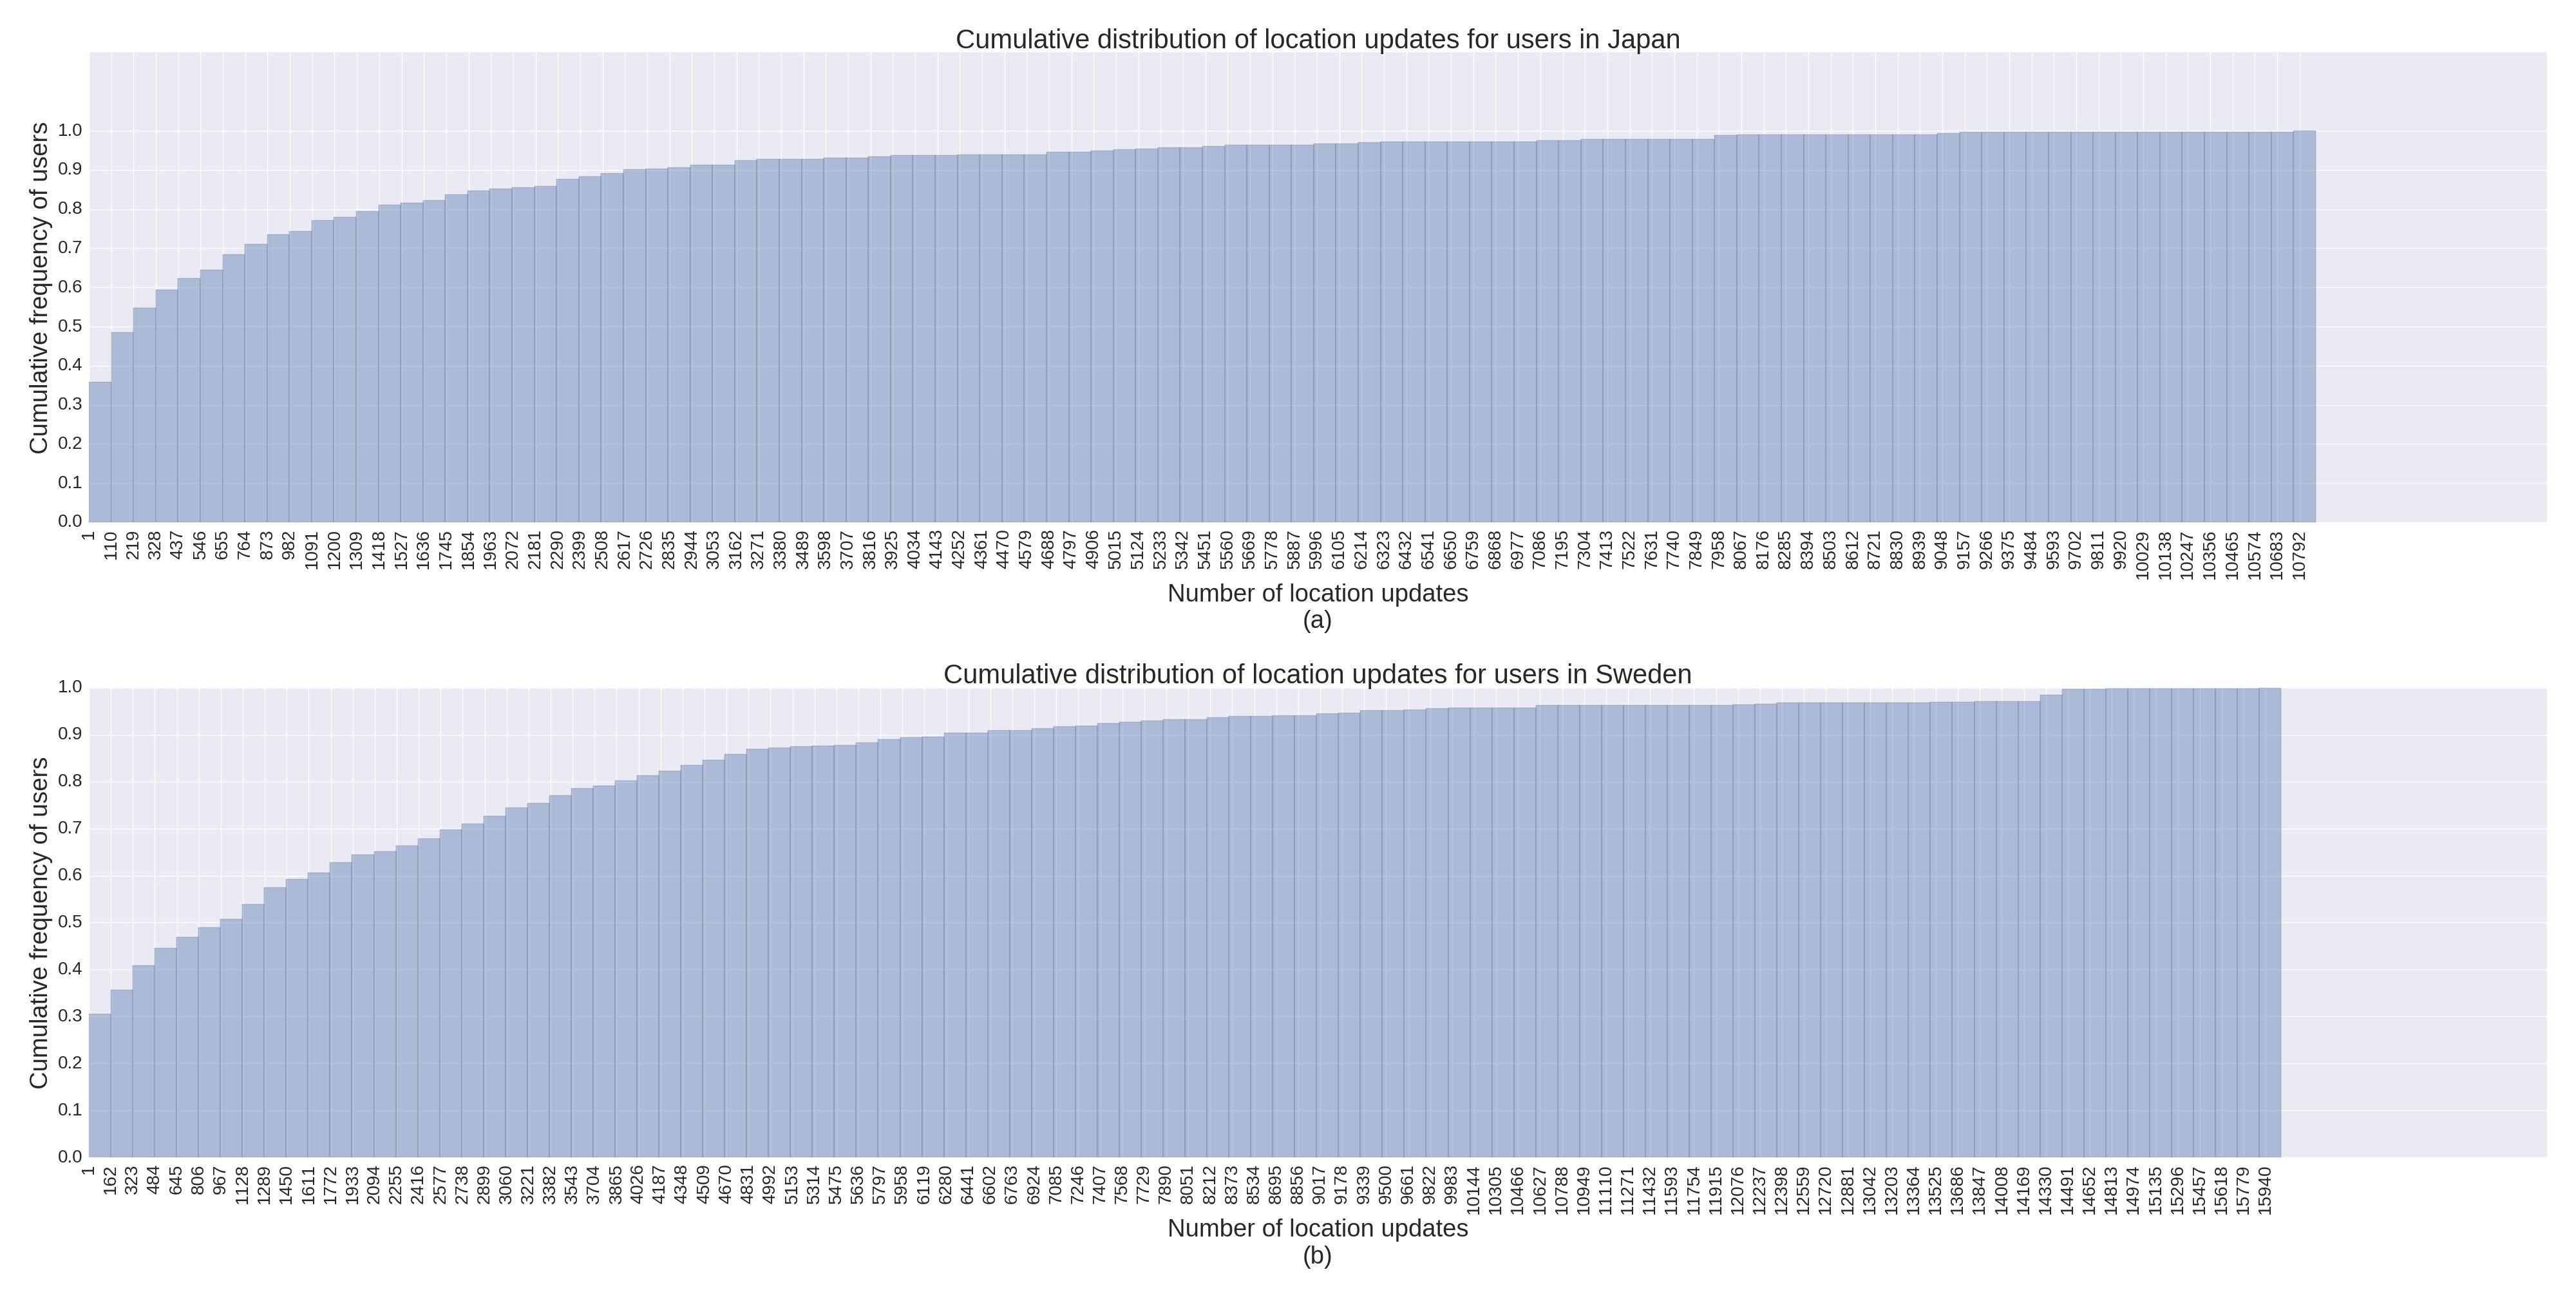
\includegraphics[scale=0.18]{cumulative_dist_loc_updates_swe_jap}
    \caption[Cumulative distribution for location update]{Cumulative distribution for location update. (a) show the cumulative distribution for all users in Japan; (b) show it for Sweden}
    \label{fig:country_cd}
\end{figure}



\begin{figure}[H]
    \centering
    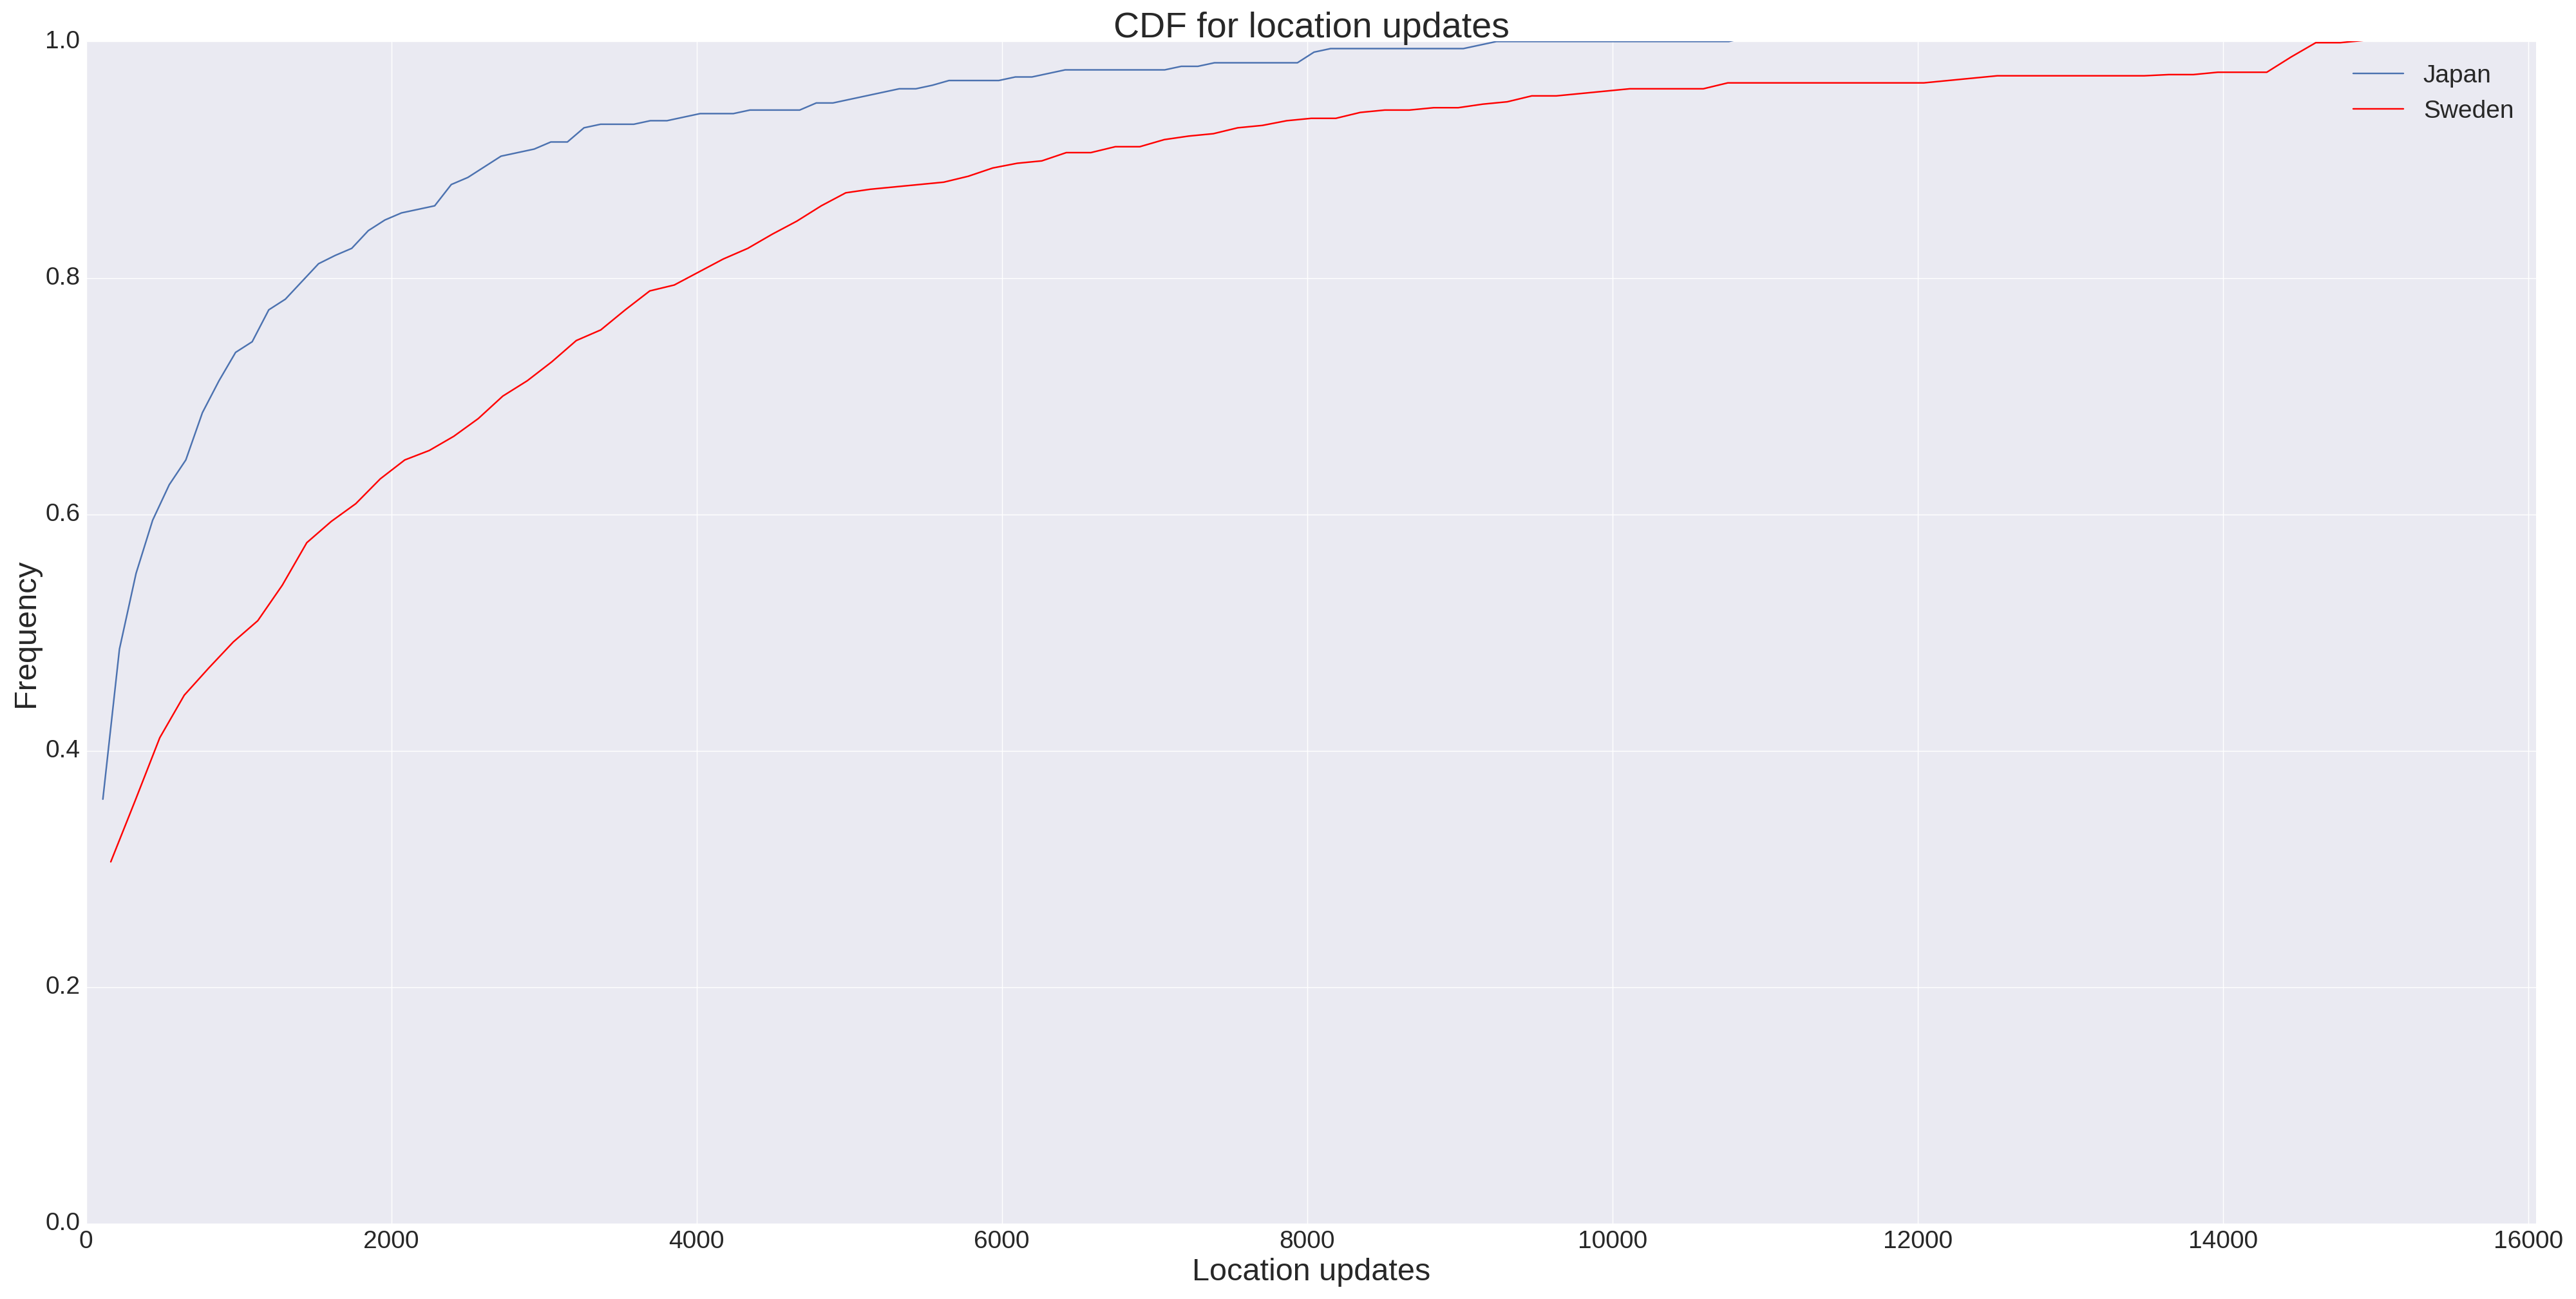
\includegraphics[scale=0.18]{cdf_location_updates_swe_jap}
    \caption{Cumulative Distribution Function (CDF) over location updates for Japan and Sweden}
    \label{fig:country_cdf}
\end{figure}

For at bedre kunne sammenligne Japan og Sverige udfra Figure \ref{fig:country_cd}, har vi plottet den Cumulative Distribution Function (CDF) for de to lande (Figure \ref{fig:country_cdf}). Plottet viser at Japan har flere brugere med få lokations opdateringer end Sverige, mens Sverige har flere opdateringer generelt. Dette kunne tyde på at data fra  Sverige vil være mere brugbart end Japan. Dog er binsize forskellig for de to plot og hvis vi sammenligner nøgleværdierne for de to lande (Table \ref{tab:stat_loc_updates}) kan vi se, at Sverige har større Q1 end Japan.

\begin{table}[htbp]
        \centering
        \small
        \setlength\tabcolsep{2pt}
        \begin{tabular}{|c|c|c|c|c|c|c|c|c|c|c|}
            \hline
                         & Japan      &   Sweden      \\[-3pt]
            \hline
                 Minimum &    0.003       &   0.002          \\
            \hline
                 Q1      &  0.081     &   0.140      \\
            \hline
                 Median  & 0.679     &   1.851      \\
            \hline
                 Mean    &  2.973   &  4.191     \\
            \hline
                 Q3      & 3.330    &   5.855     \\
            \hline
                 Maximum &  32.744 &  28.820     \\
            \hline
                 IQR     &  3.349   &  5.715      \\
            \hline
            
        \end{tabular}
        \caption{Quantiles and mean over location updates for Japan and Sweden per user} %add this between 'caption' and '{...' for new text in listing of tables: [New caption text only for listing of tables]
        \label{tab:stat_loc_updates}
\end{table}


En ting er at kigge på antal lokations opdateringer og se hvordan de er distribueret blandt brugerne i det pågældende land, men det er også interessant at se hvordan opdateringerne er distribueret henover de 3 måneder vi har med at gøre. Er det ligeligt fordelt? Står en enekelt måned for det hele? Er der forskelt på de to lande? Til dette har vi valgt at visualisere dette ved brug af Heatmaps (Figure \ref{fig:heatmap_jap} p.  \pageref{fig:heatmap_jap} and Figure \ref{fig:heatmap_swe} p. \pageref{fig:heatmap_swe}). 
\begin{figure}[H]
    \centering
    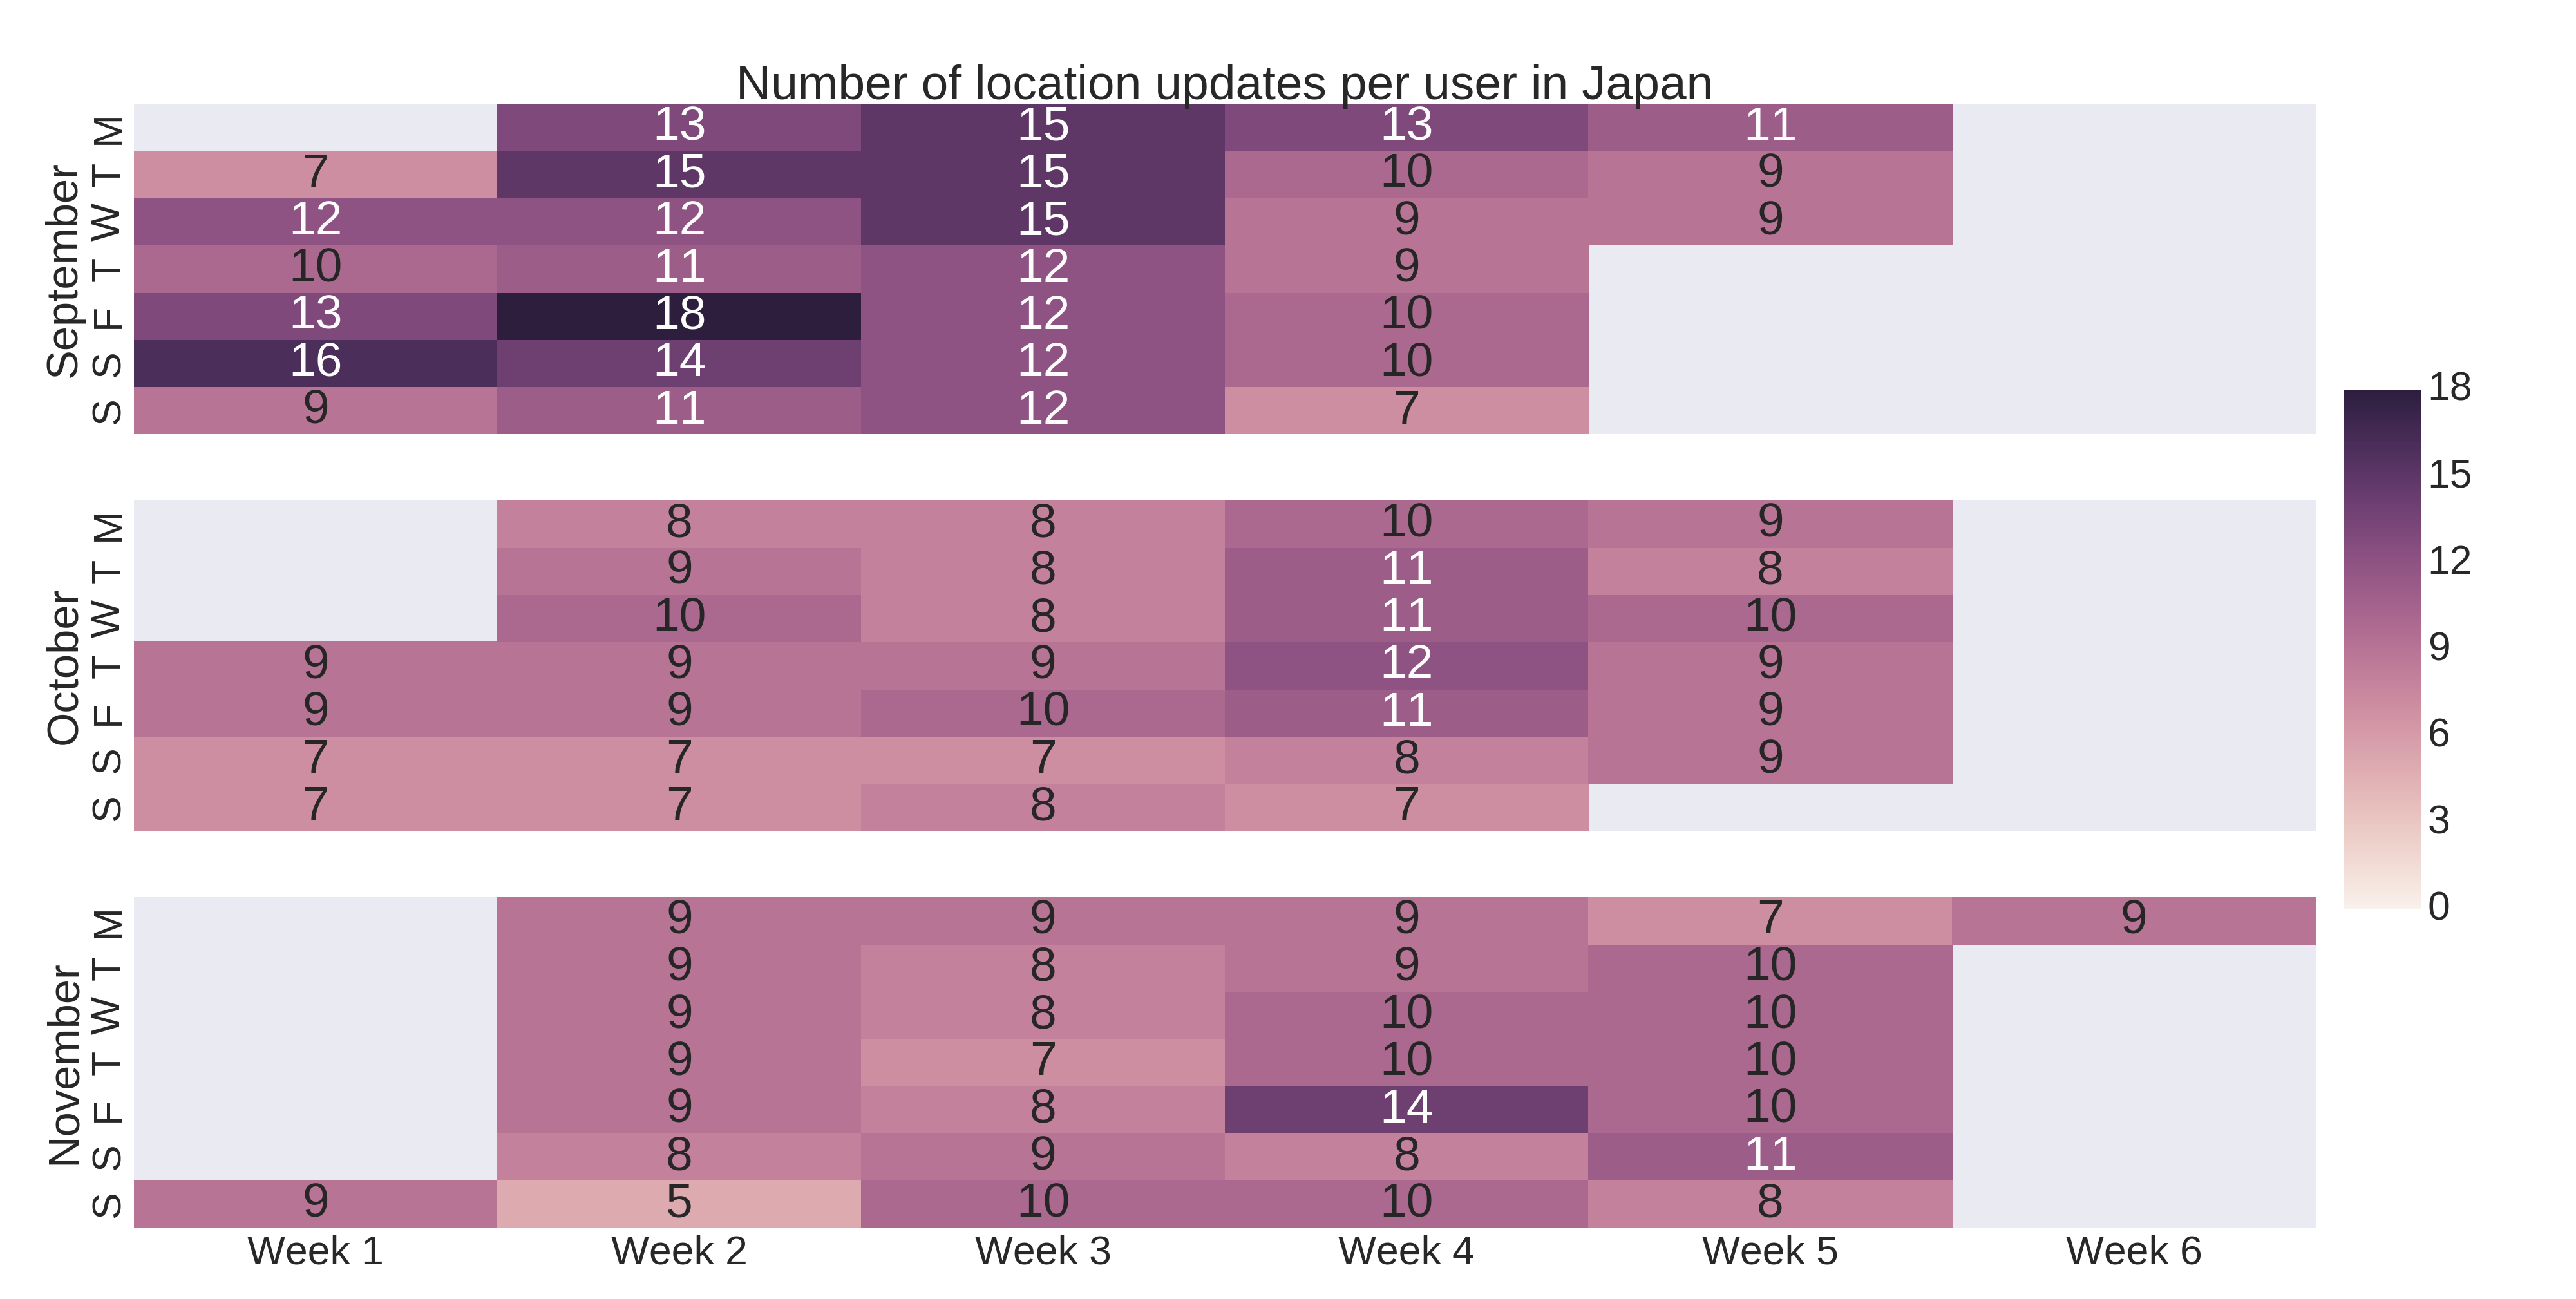
\includegraphics[scale=0.18]{heatmap_location_updates_japan}
    \caption{Heatmap for location updates over the 3 month period in Japan}
    \label{fig:heatmap_jap}
\end{figure}


\begin{figure}[H]
    \centering
    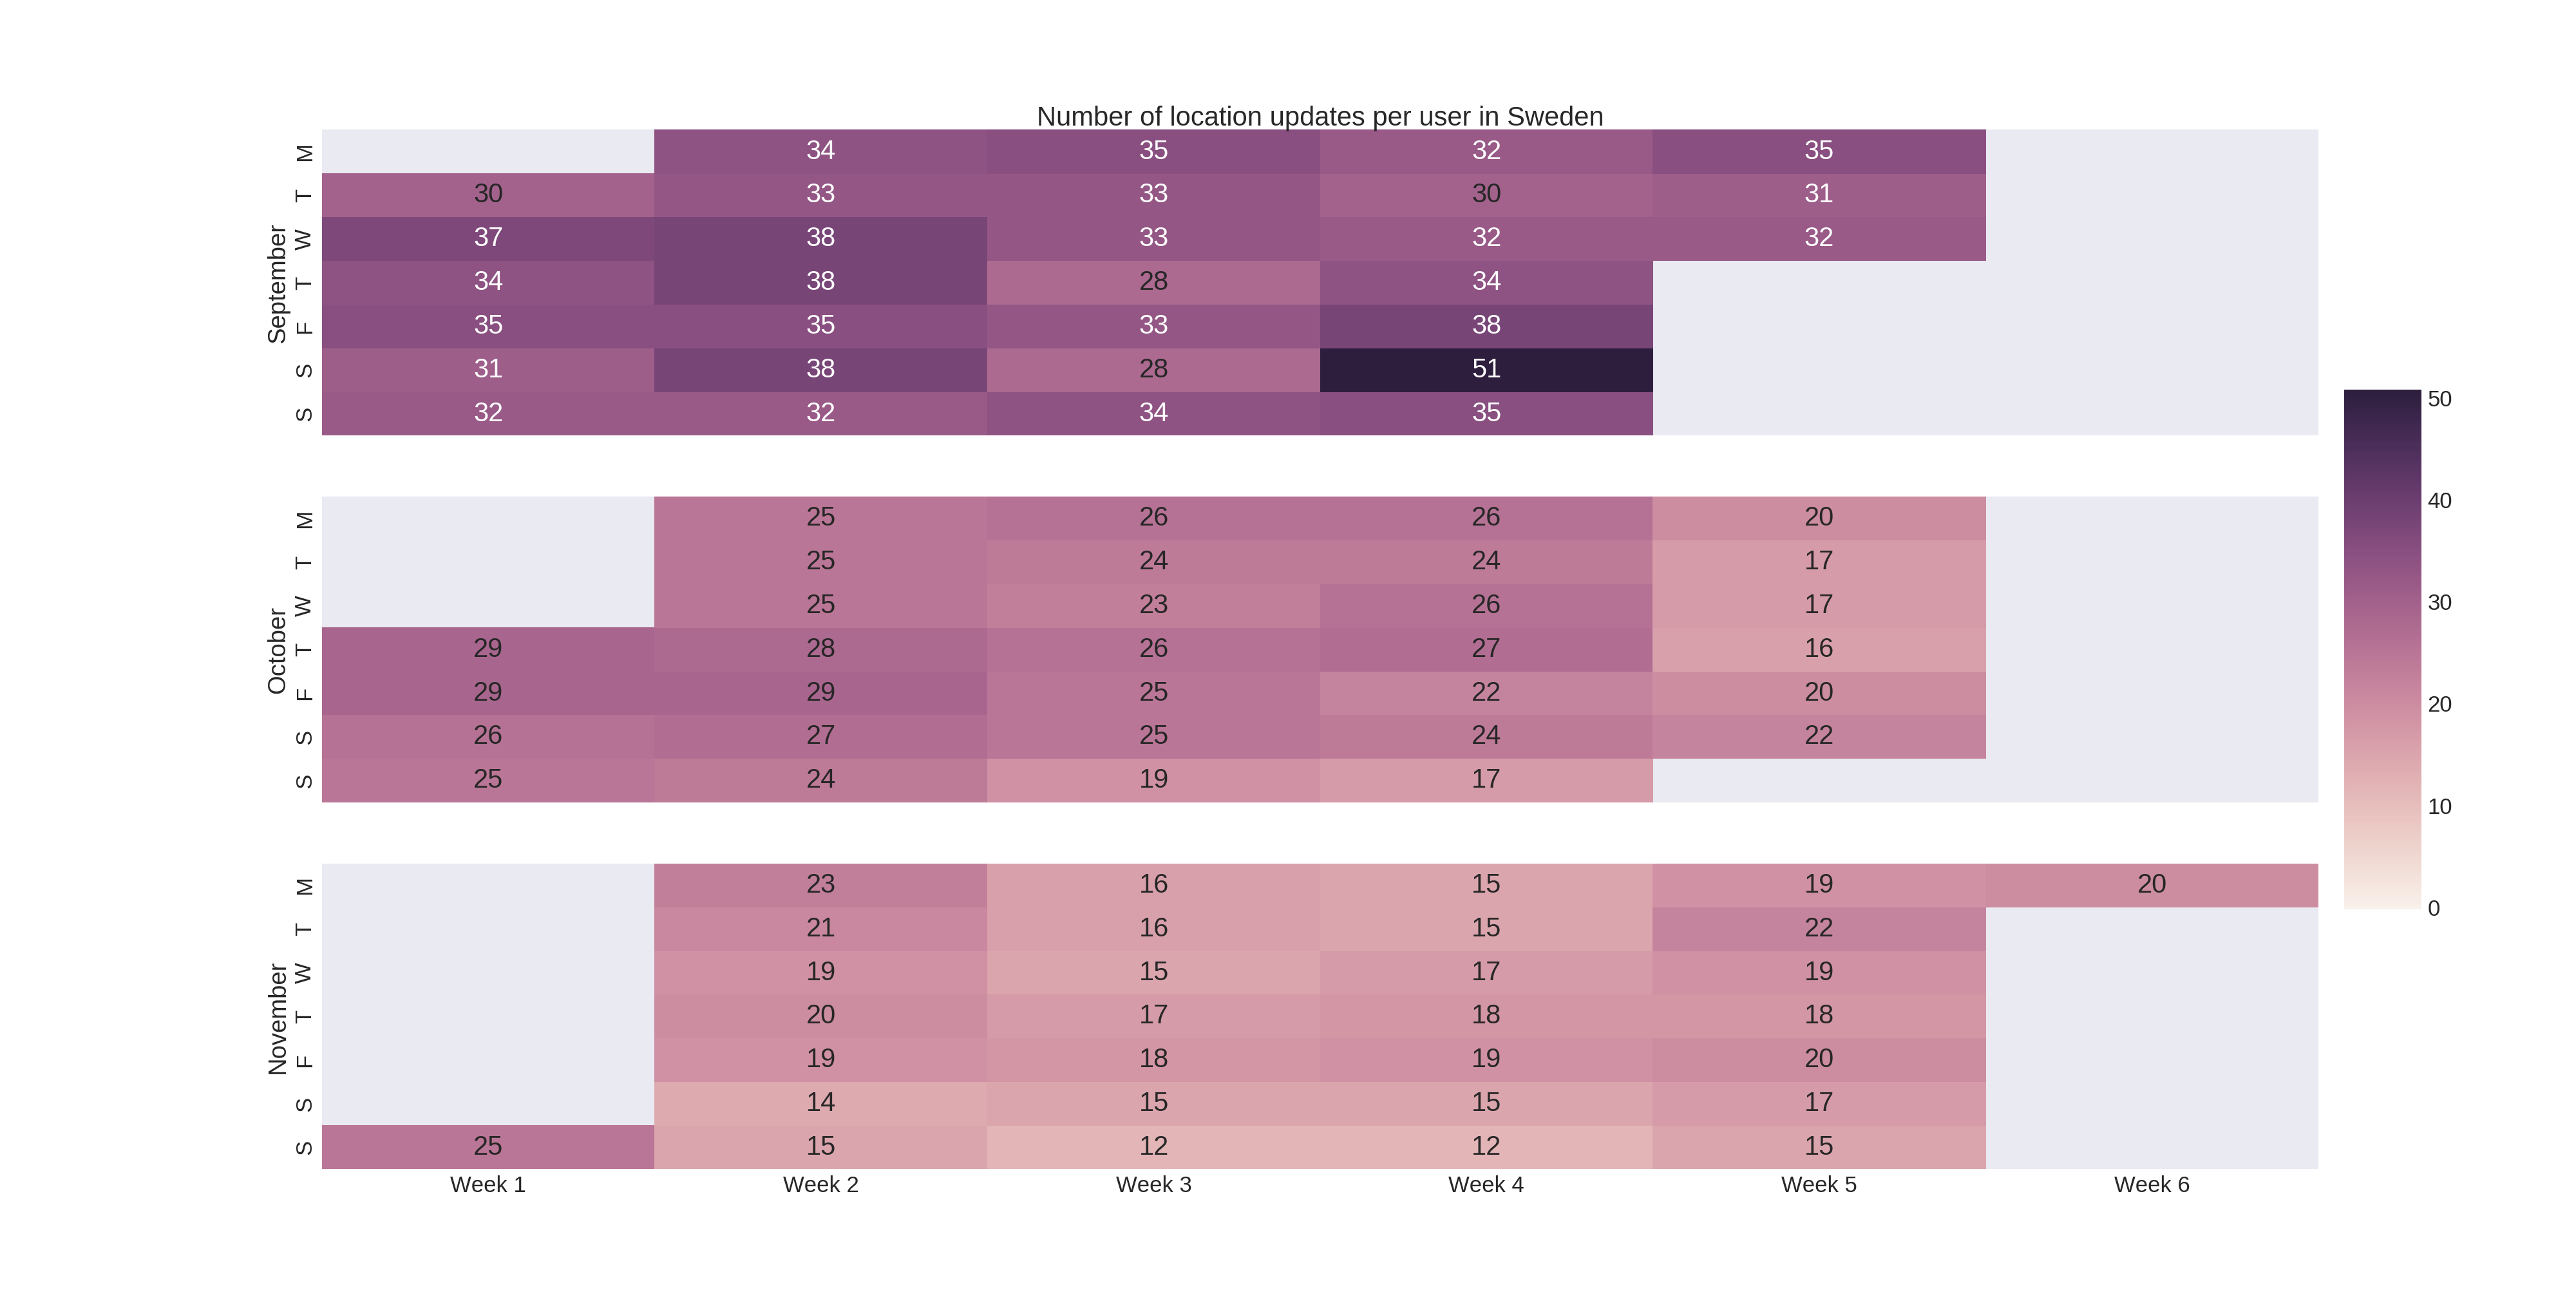
\includegraphics[scale=0.18]{heatmap_location_updates_sweden}
    \caption{Heatmap for location updates over the 3 month period in Sweden}
    \label{fig:heatmap_swe}
\end{figure}



Som man kan er der lidt færrer lande end det vi tidligere skyldtes. Dette 

Our work will focus on the location updates from Japan. There is 332 users in Japan for which we have location updates.
When training our classifier we divided the dataset into three parts where each corresponded to a month.

Japan locations for September: 340198
Japan locations for October: 208242
Japan locations for November: 102442

%\subsection{App og homophily del}


Over disse 3 måneder blev der indsamlet 2.665.893 geolokation lokations opdaterings, som er vores primær data. 

When we got the dataset it was stored in three folders, one for each month (9, 10, 11) and within each folder were multiple chunks of data in Apache Avro format\cite{apacheavro}, which we learned is a data serialization framework for Hadoop similar to the JSON format. The chunks were contained in folders bearing the number for each month, however we learned they were sorted by when the server had received the data packet containing the location from the phone and not when the phone had registered the location. The app is storing the collected data on the users phone for a maximum of one month, if the data is not uploaded within a month it is discarded. This approach to data collection means the month folders can contain location updates from the previous month as well.


\subsubsection{Periode 2}